\section{Results} %4.4
\label{section4.4}
\subsection{Results and Analysis} %4.4.1
The implement results are as follows. Figure~\ref{4_4_1_result1} shows all the acceptable signals.

\begin{figure}[htbp]
\centering
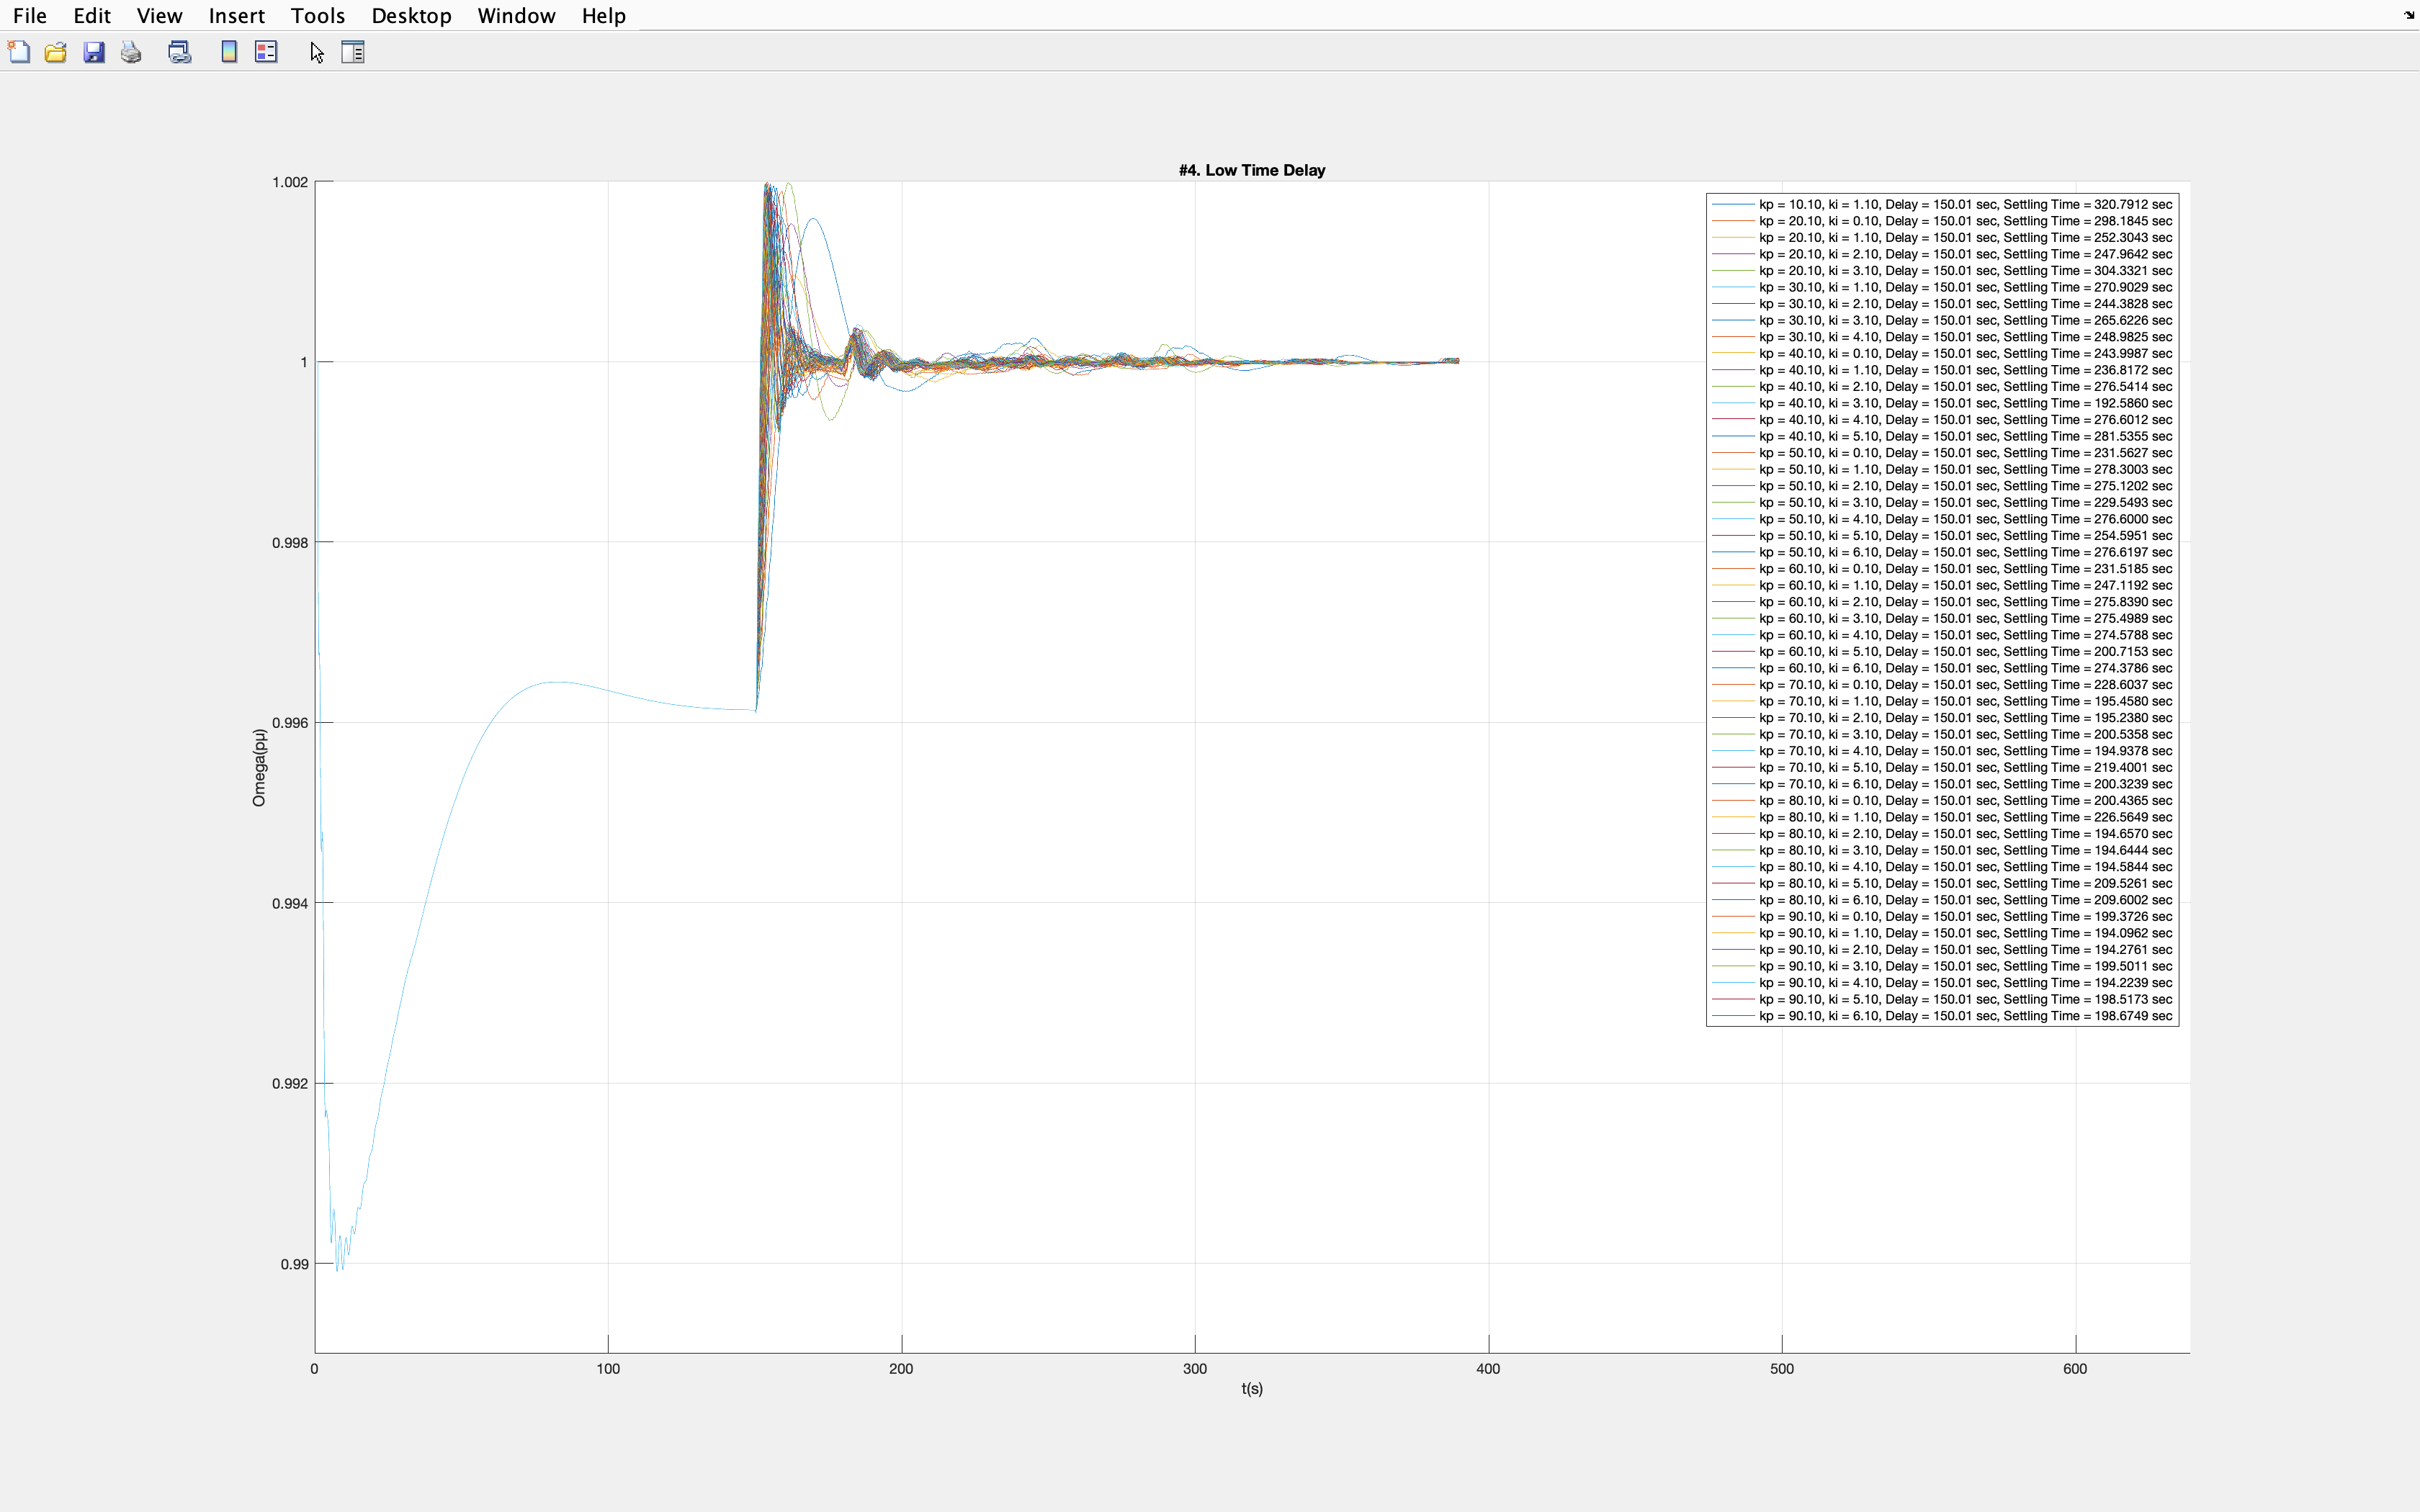
\includegraphics[width = .819\textwidth]{figure/4_4_1_result1.png}
\caption{MATLAB plot: all the acceptable signals.}
\label{4_4_1_result1}
\end{figure}

From Figure~\ref{4_4_1_result1}, we can roughly draw a conclusion that the signals are indeed within a reasonable range and it seems that they have finally reached the nominal value.  

However, we need to check further by choosing one of the signals. For instance, I choose the signal whose kp is 90.1 and ki is 7.1. The reason I choose this signal is that it is located at the borderline. Results are as follows.  

\begin{figure}[htbp]
\centering
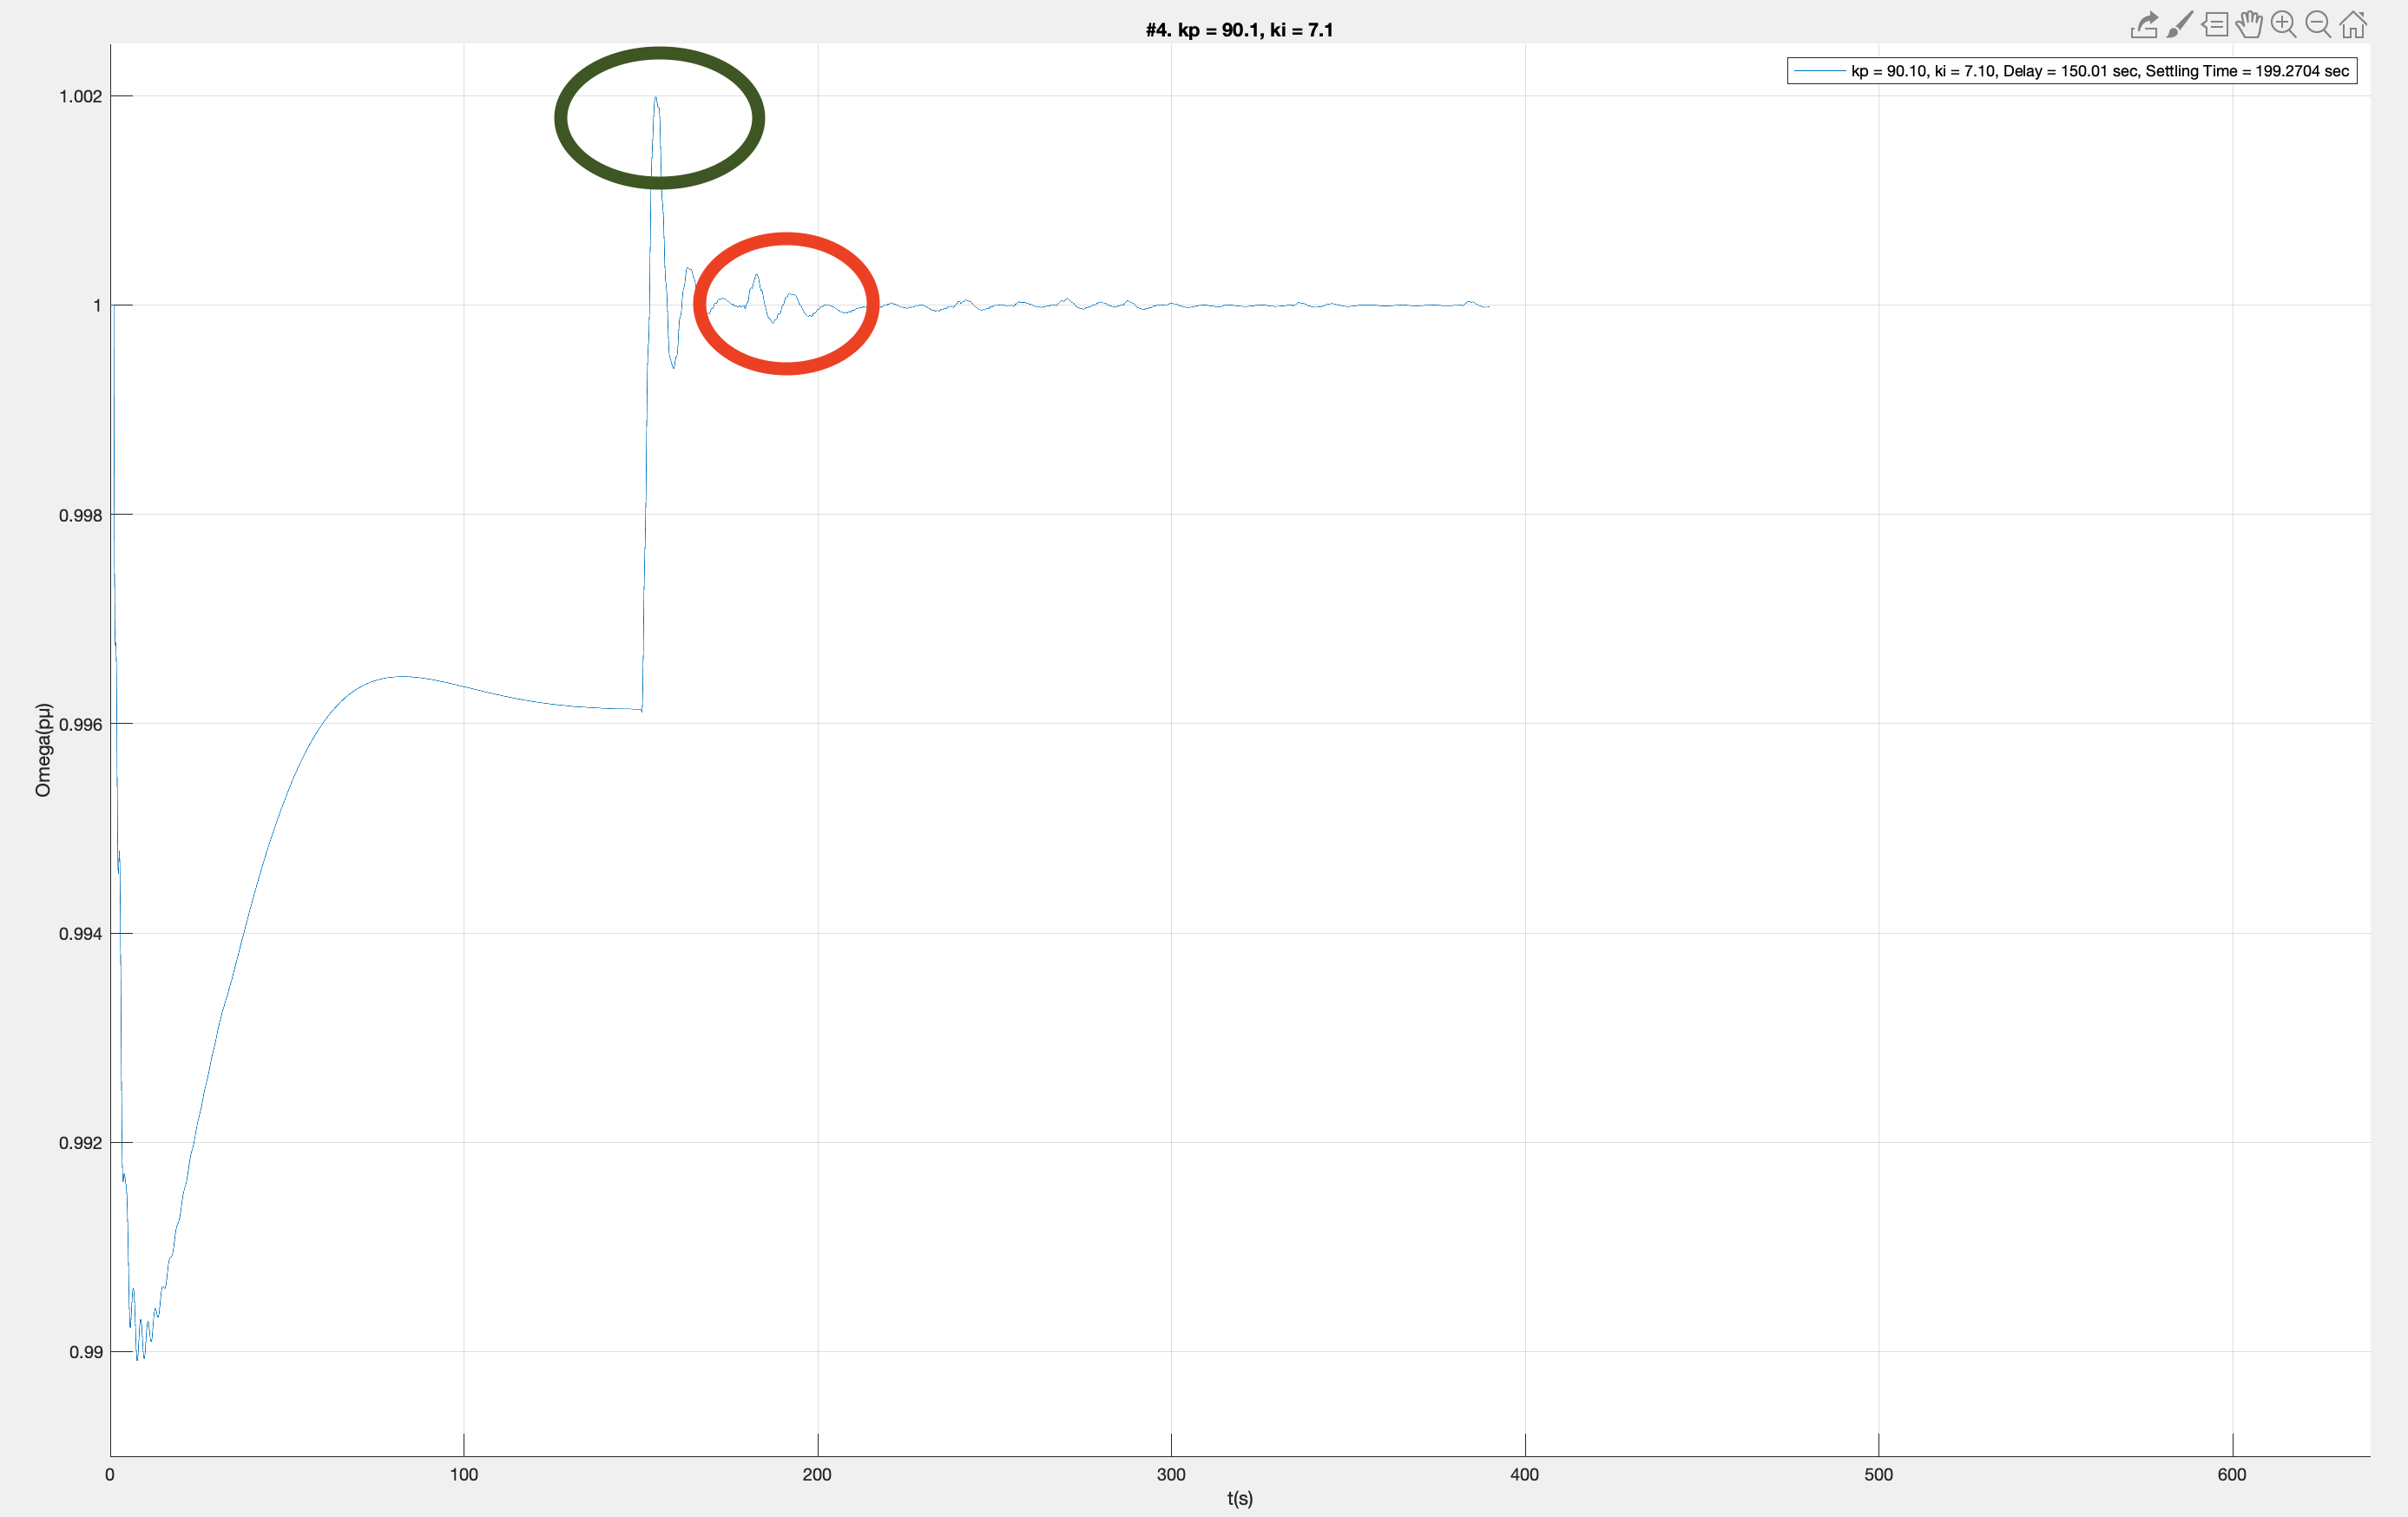
\includegraphics[width = .819\textwidth]{figure/4_4_1_result2.png}
\caption{The whole picture: whether the controlled signal meet the conditions: frequency limit and settling condition}
\label{4_4_1_result2}
\end{figure}

From the Figure~\ref{4_4_1_result2}, we can see that the overshoot does not exceed 1.002 obviously. But for the settling time, we can not make any conclusion until we see the details.  


\begin{figure}[htbp]
\centering
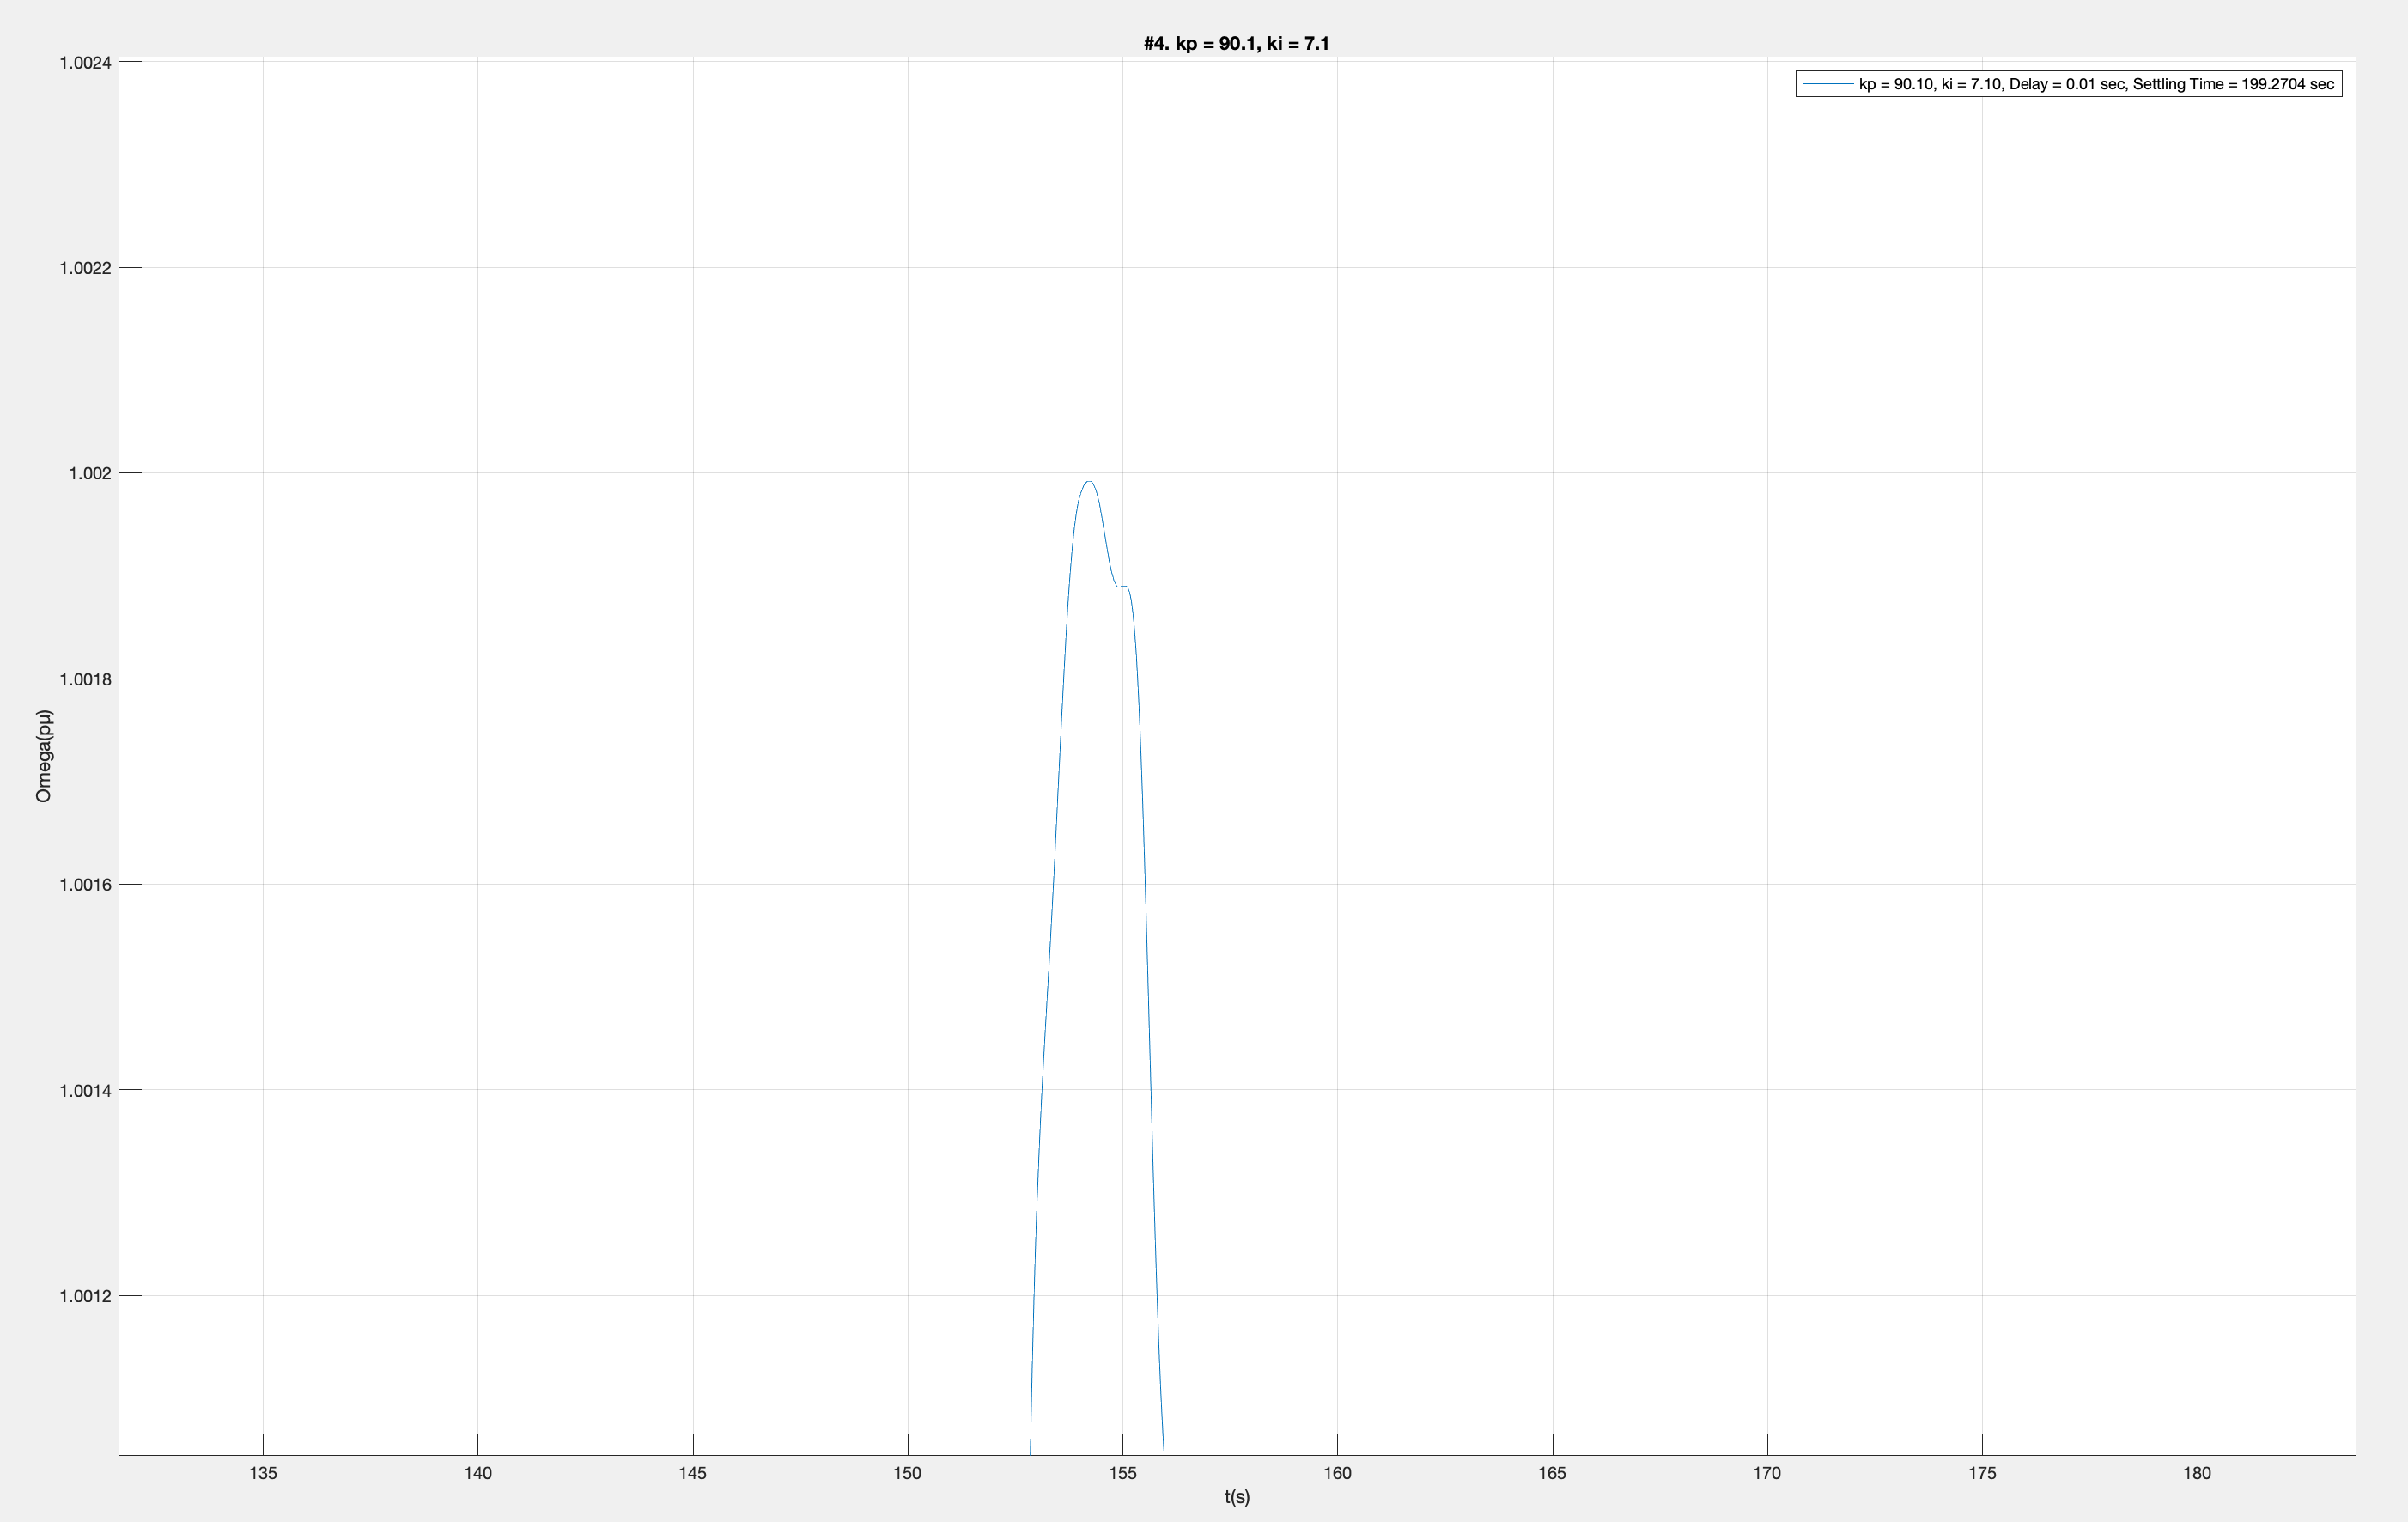
\includegraphics[width = .819\textwidth]{figure/4_4_1_result3.png}
\caption{Details: check frequency limit.}
\label{4_4_1_result3}
\end{figure}

From Figure~\ref{4_4_1_result3}, we can judge that its overshoot does not exceed the maximum allowable value, i.e. 1.002 $p\mu$, after the signal settled. 

\begin{figure}[htbp]
\centering
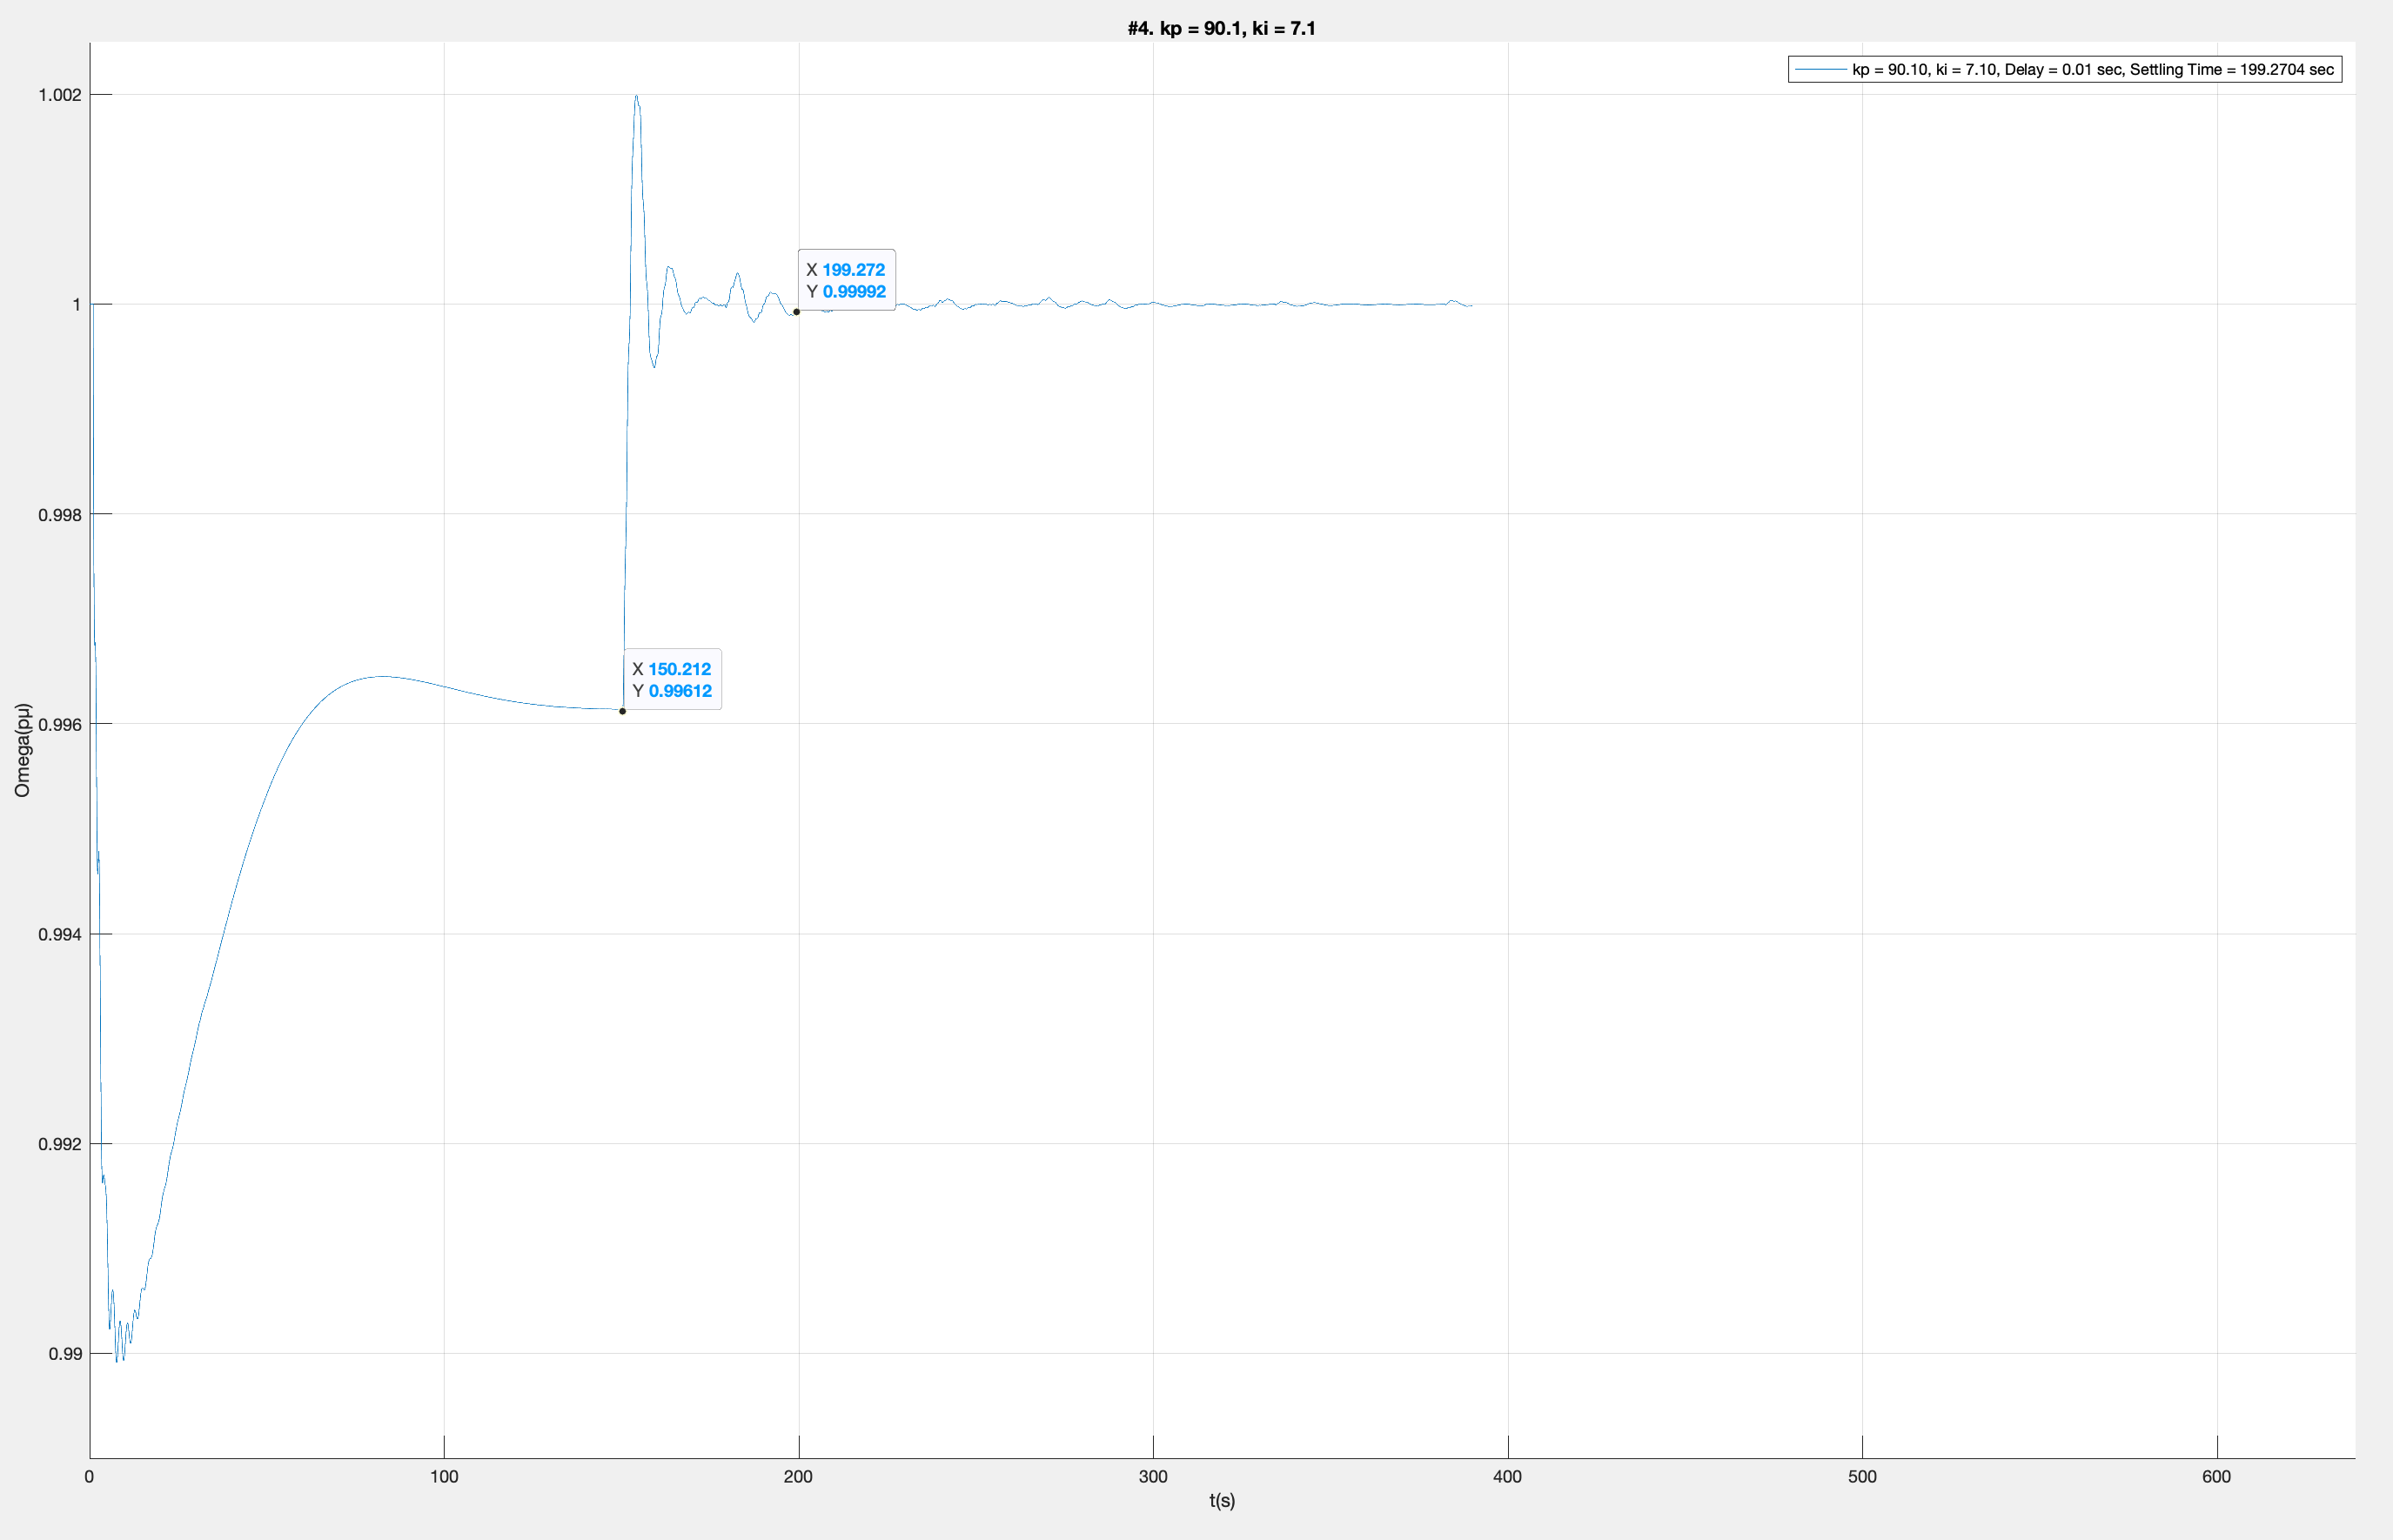
\includegraphics[width = .819\textwidth]{figure/4_4_1_result4.png}
\caption{Details: check settling condition.}
\label{4_4_1_result4}
\end{figure}


From Figure~\ref{4_4_1_result4}, we find that, after the signal settled, the signal is between the settling time threshold, i.e. 0.9998 $p\mu$ and 1.0002 $p\mu$. 


With the prove above, we can finally say that our assumed acceptable simulation results are acceptable. 

Next, we show you the relationship between kp and ki. 

\begin{table*}[htbp]
\centering
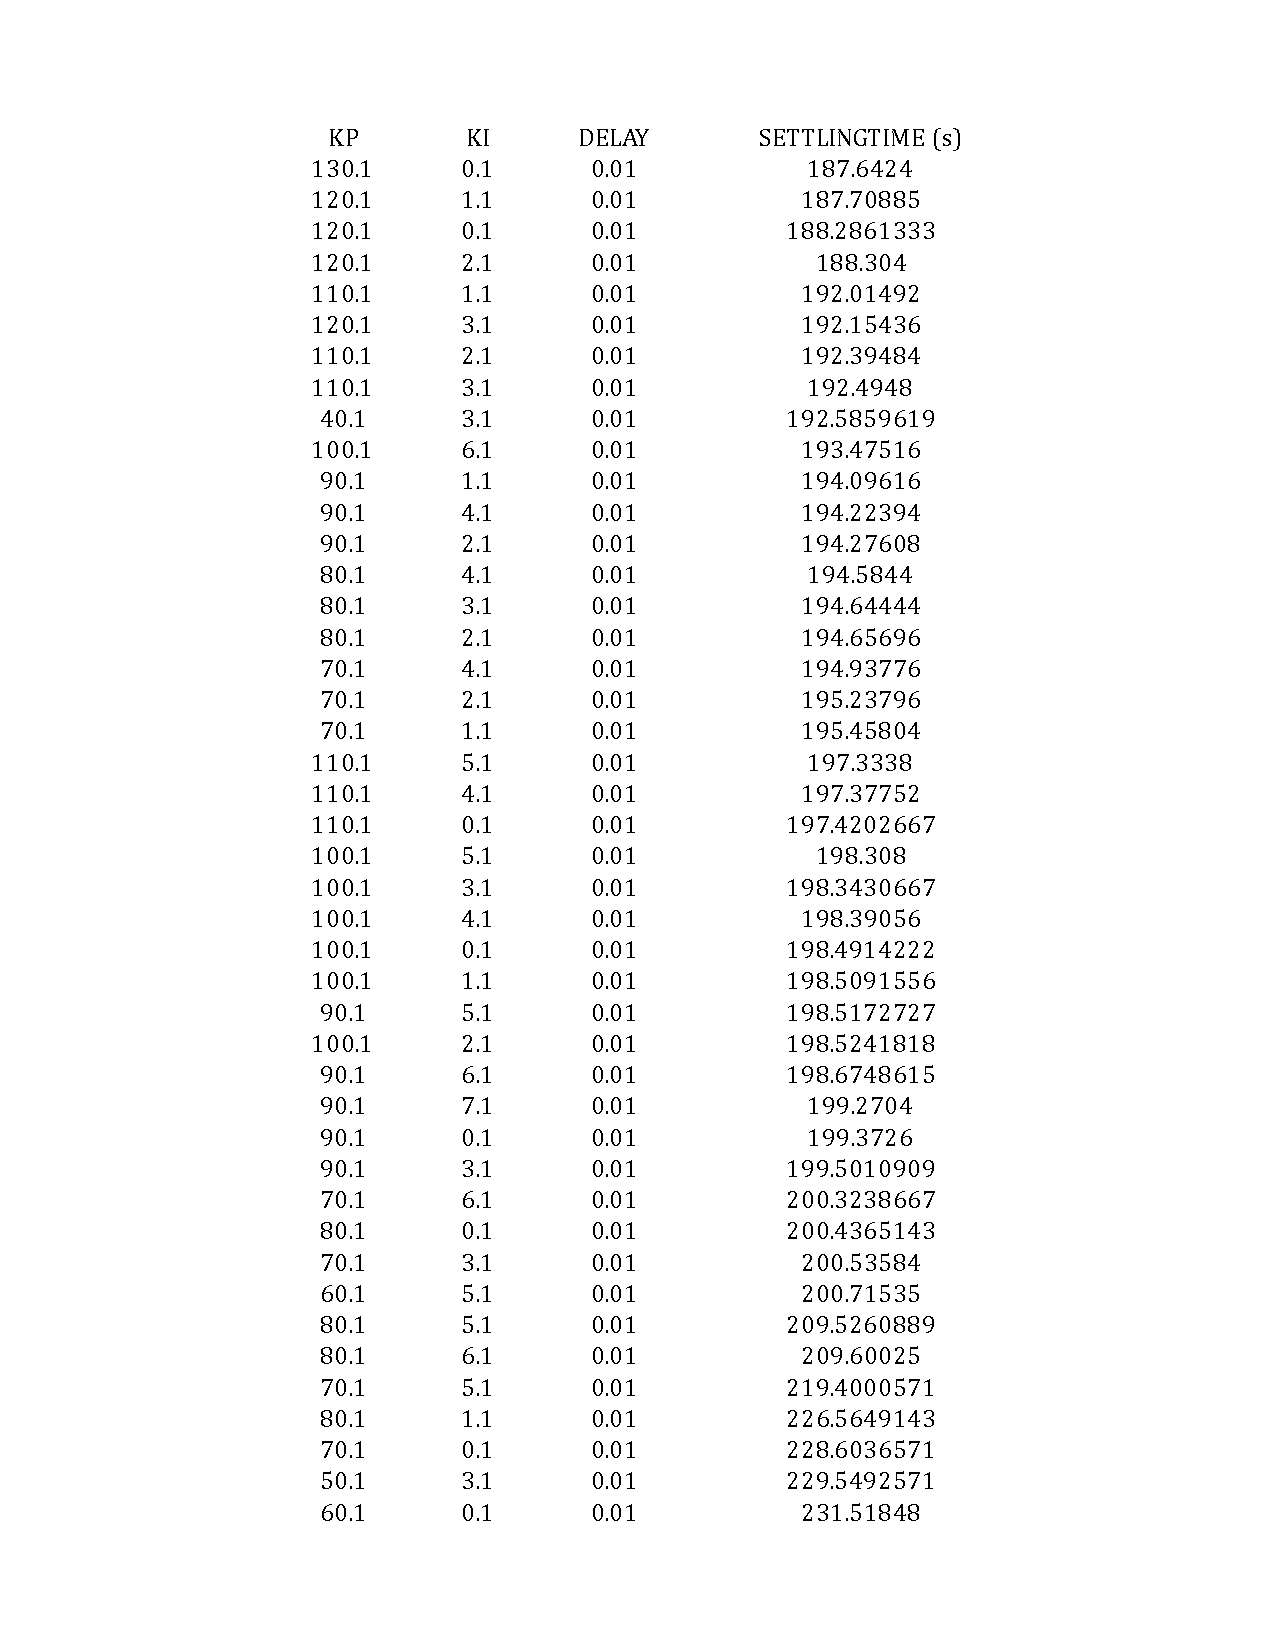
\includegraphics[width = \textwidth]{figure/4_4_1_table.pdf}
\caption{Part of the acceptable results ranked by settling time.}
\label{4_4_1_table}
\end{table*}

 Table~\ref{4_4_1_table} shows the parameters that make up the acceptable signals, i.e. kp, ki, delay and settling time. It has ranked by the settling time.  

\begin{figure}[htbp]
\centering
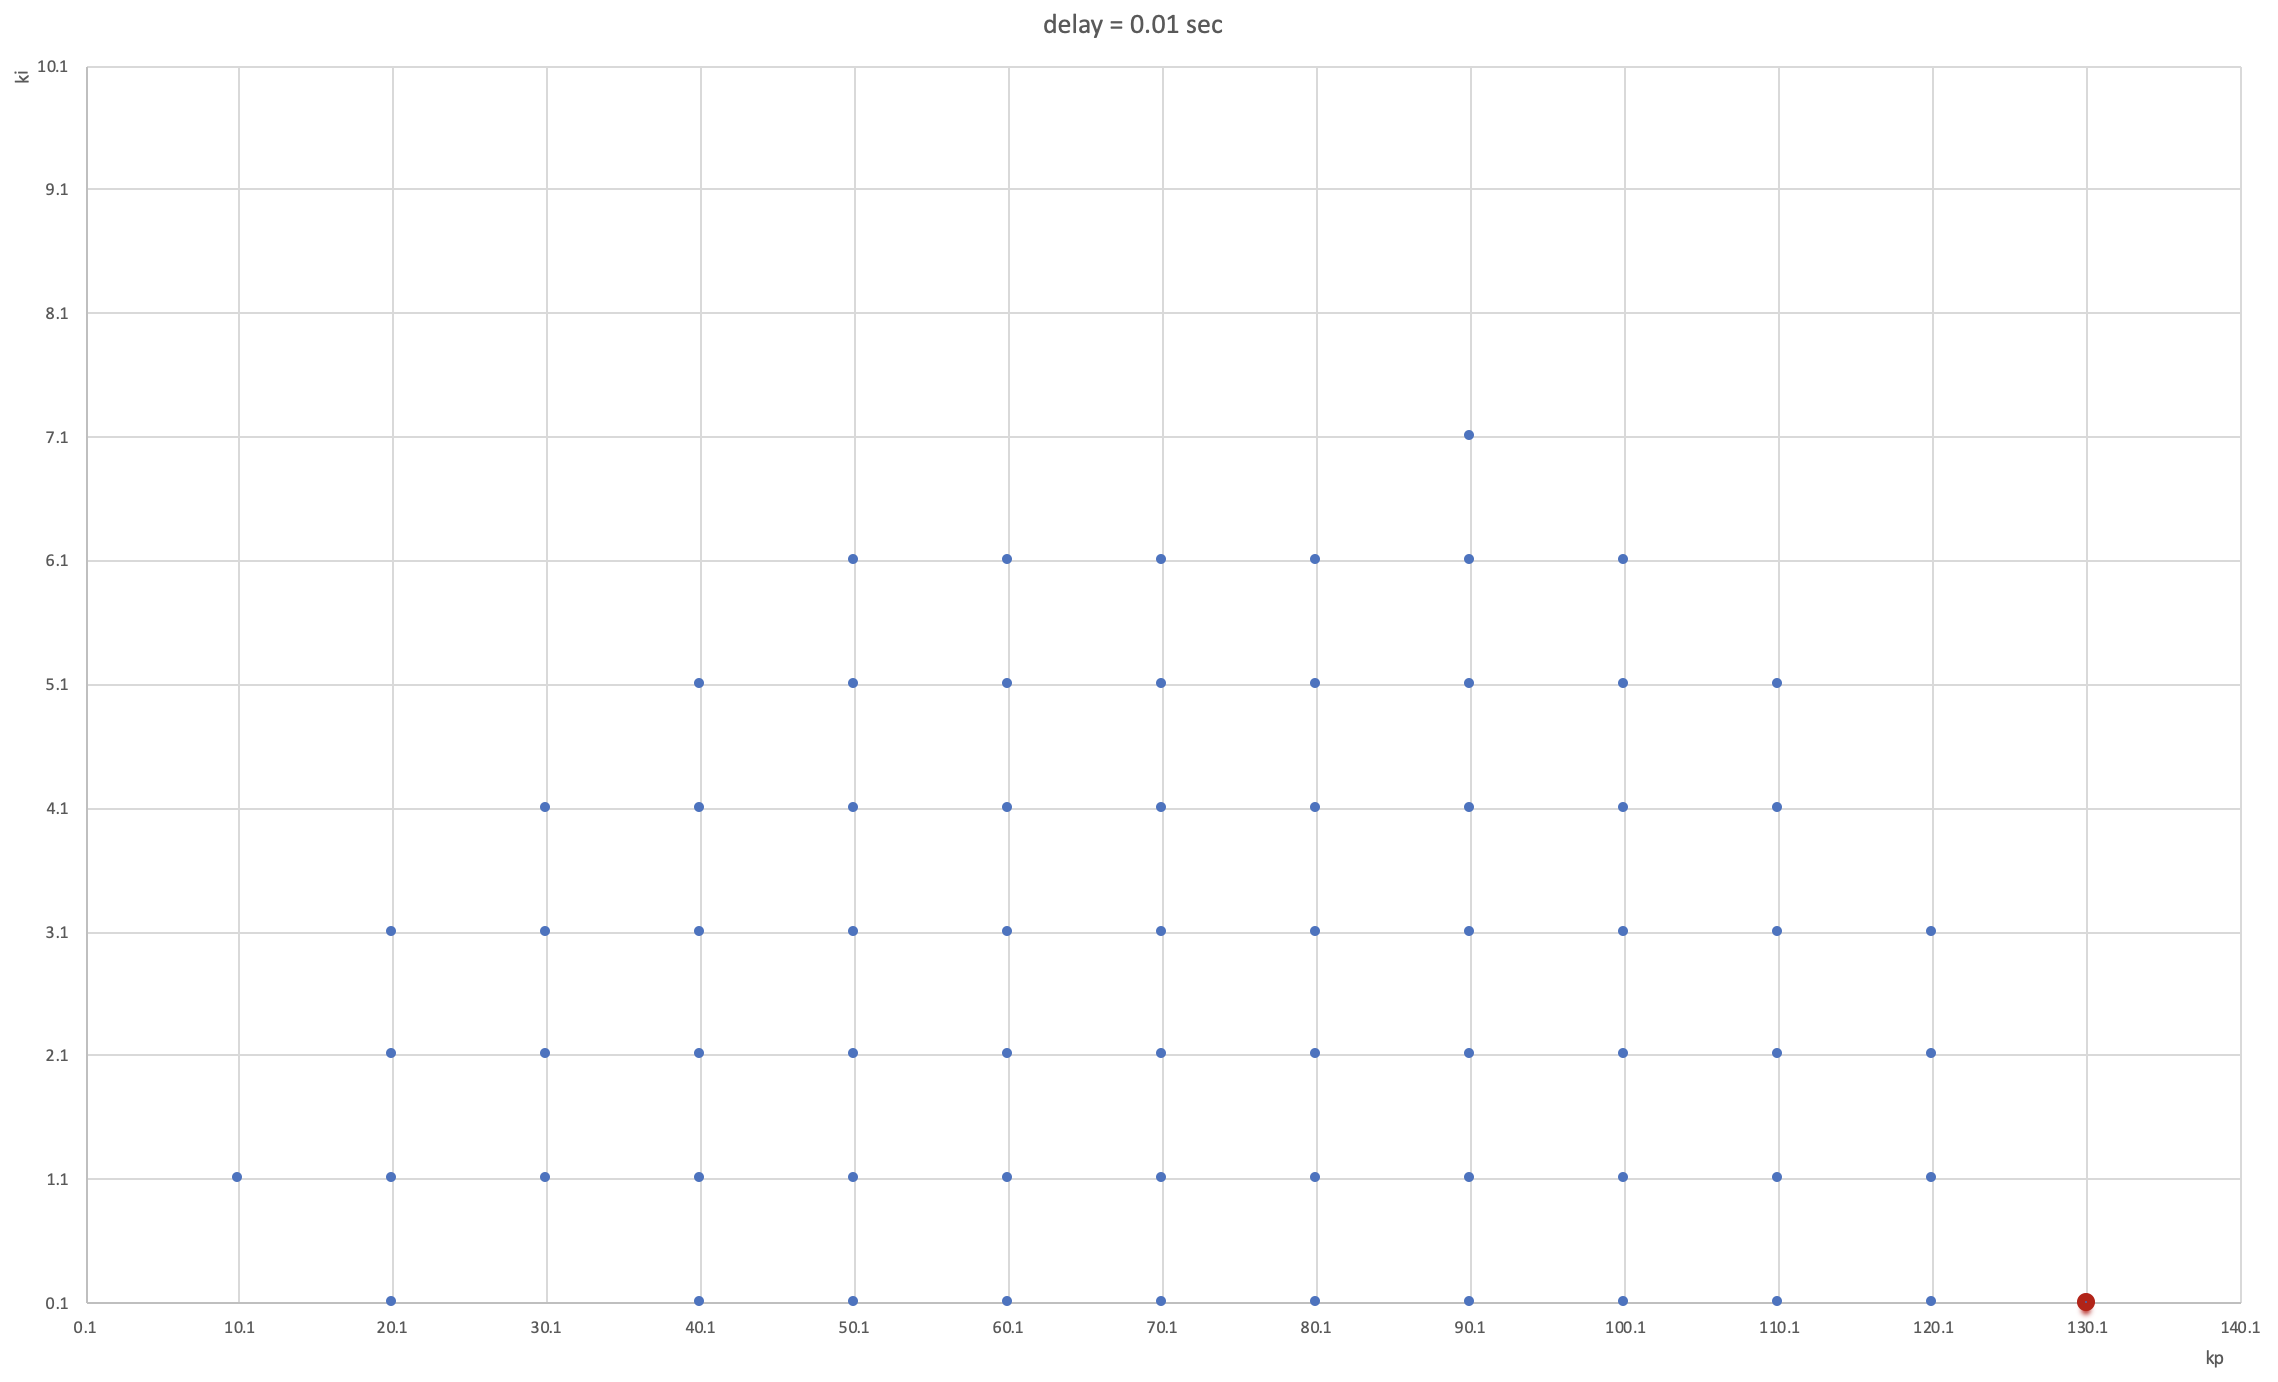
\includegraphics[width = .819\textwidth]{figure/4_4_1_2d.png}
\caption{2D plot: All the acceptable tuning results in low time delay.}
\label{4_4_1_2d}
\end{figure}

Table~\ref{4_4_1_2d} draws a 2D graph where kp is horizontal axis and ki is vertical axis. Besides, we highlight the point which gives the minimum settling time as a reference. 

Analysing the Table~\ref{4_4_1_2d}, we can find: 

\begin{itemize}
\item The 2D graph shows a clear borderline which separates the acceptable results and unacceptable results. This is in line with the previous expectation from section~\ref{section4.2}; 

\item The best point is (130.1, 0.1); 

\item The best point is in the borderline.  This is not in line with the previous expectation from section~\ref{section4.2}; 

\item The best point’s kp value is too large. This is not in line with the previous expectation from section~\ref{section4.2}; 

\item The best point's ki value is not too large.  This is in line with the previous expectation from section~\ref{section4.2}; 

\item The worst point, i.e. kp is 10.1 and ki is 1.1, shows in the borderline. This is in line with the previous expectation from section~\ref{section4.2}. 
\end{itemize}

Although, for the best point, its kp is large enough to keep the signal approaching the settling status as fast as possible, it is dangerous that it would be removed by a higher time delay. 

However, the best point's ki value is 0.1, which is “unexpected” before.  

There are two explanations for this small ki value. The first explanation is that this “small” ki value is not small enough or is not the smallest because it is assumed that 0.1 is the minimum value of the range of ki at the beginning of the simulation. We do not need to find the real limit value of ki in this case because it will increase the amount of computation by an order of magnitude. There might be acceptable results whose kp is smaller than 0.1 but it is not necessary to find them in this case.  

Another explanation is that the function of the I-term is to help fixing the steady-state error. In fact, steady-state error will not be always shown if only there is a suitable kp being tuned. Besides, a larger ki will produce more oscillations and it makes a longer settling time.  


\subsection{The Best Tuning Signal} %4.4.2

\begin{figure}[htbp]
\centering
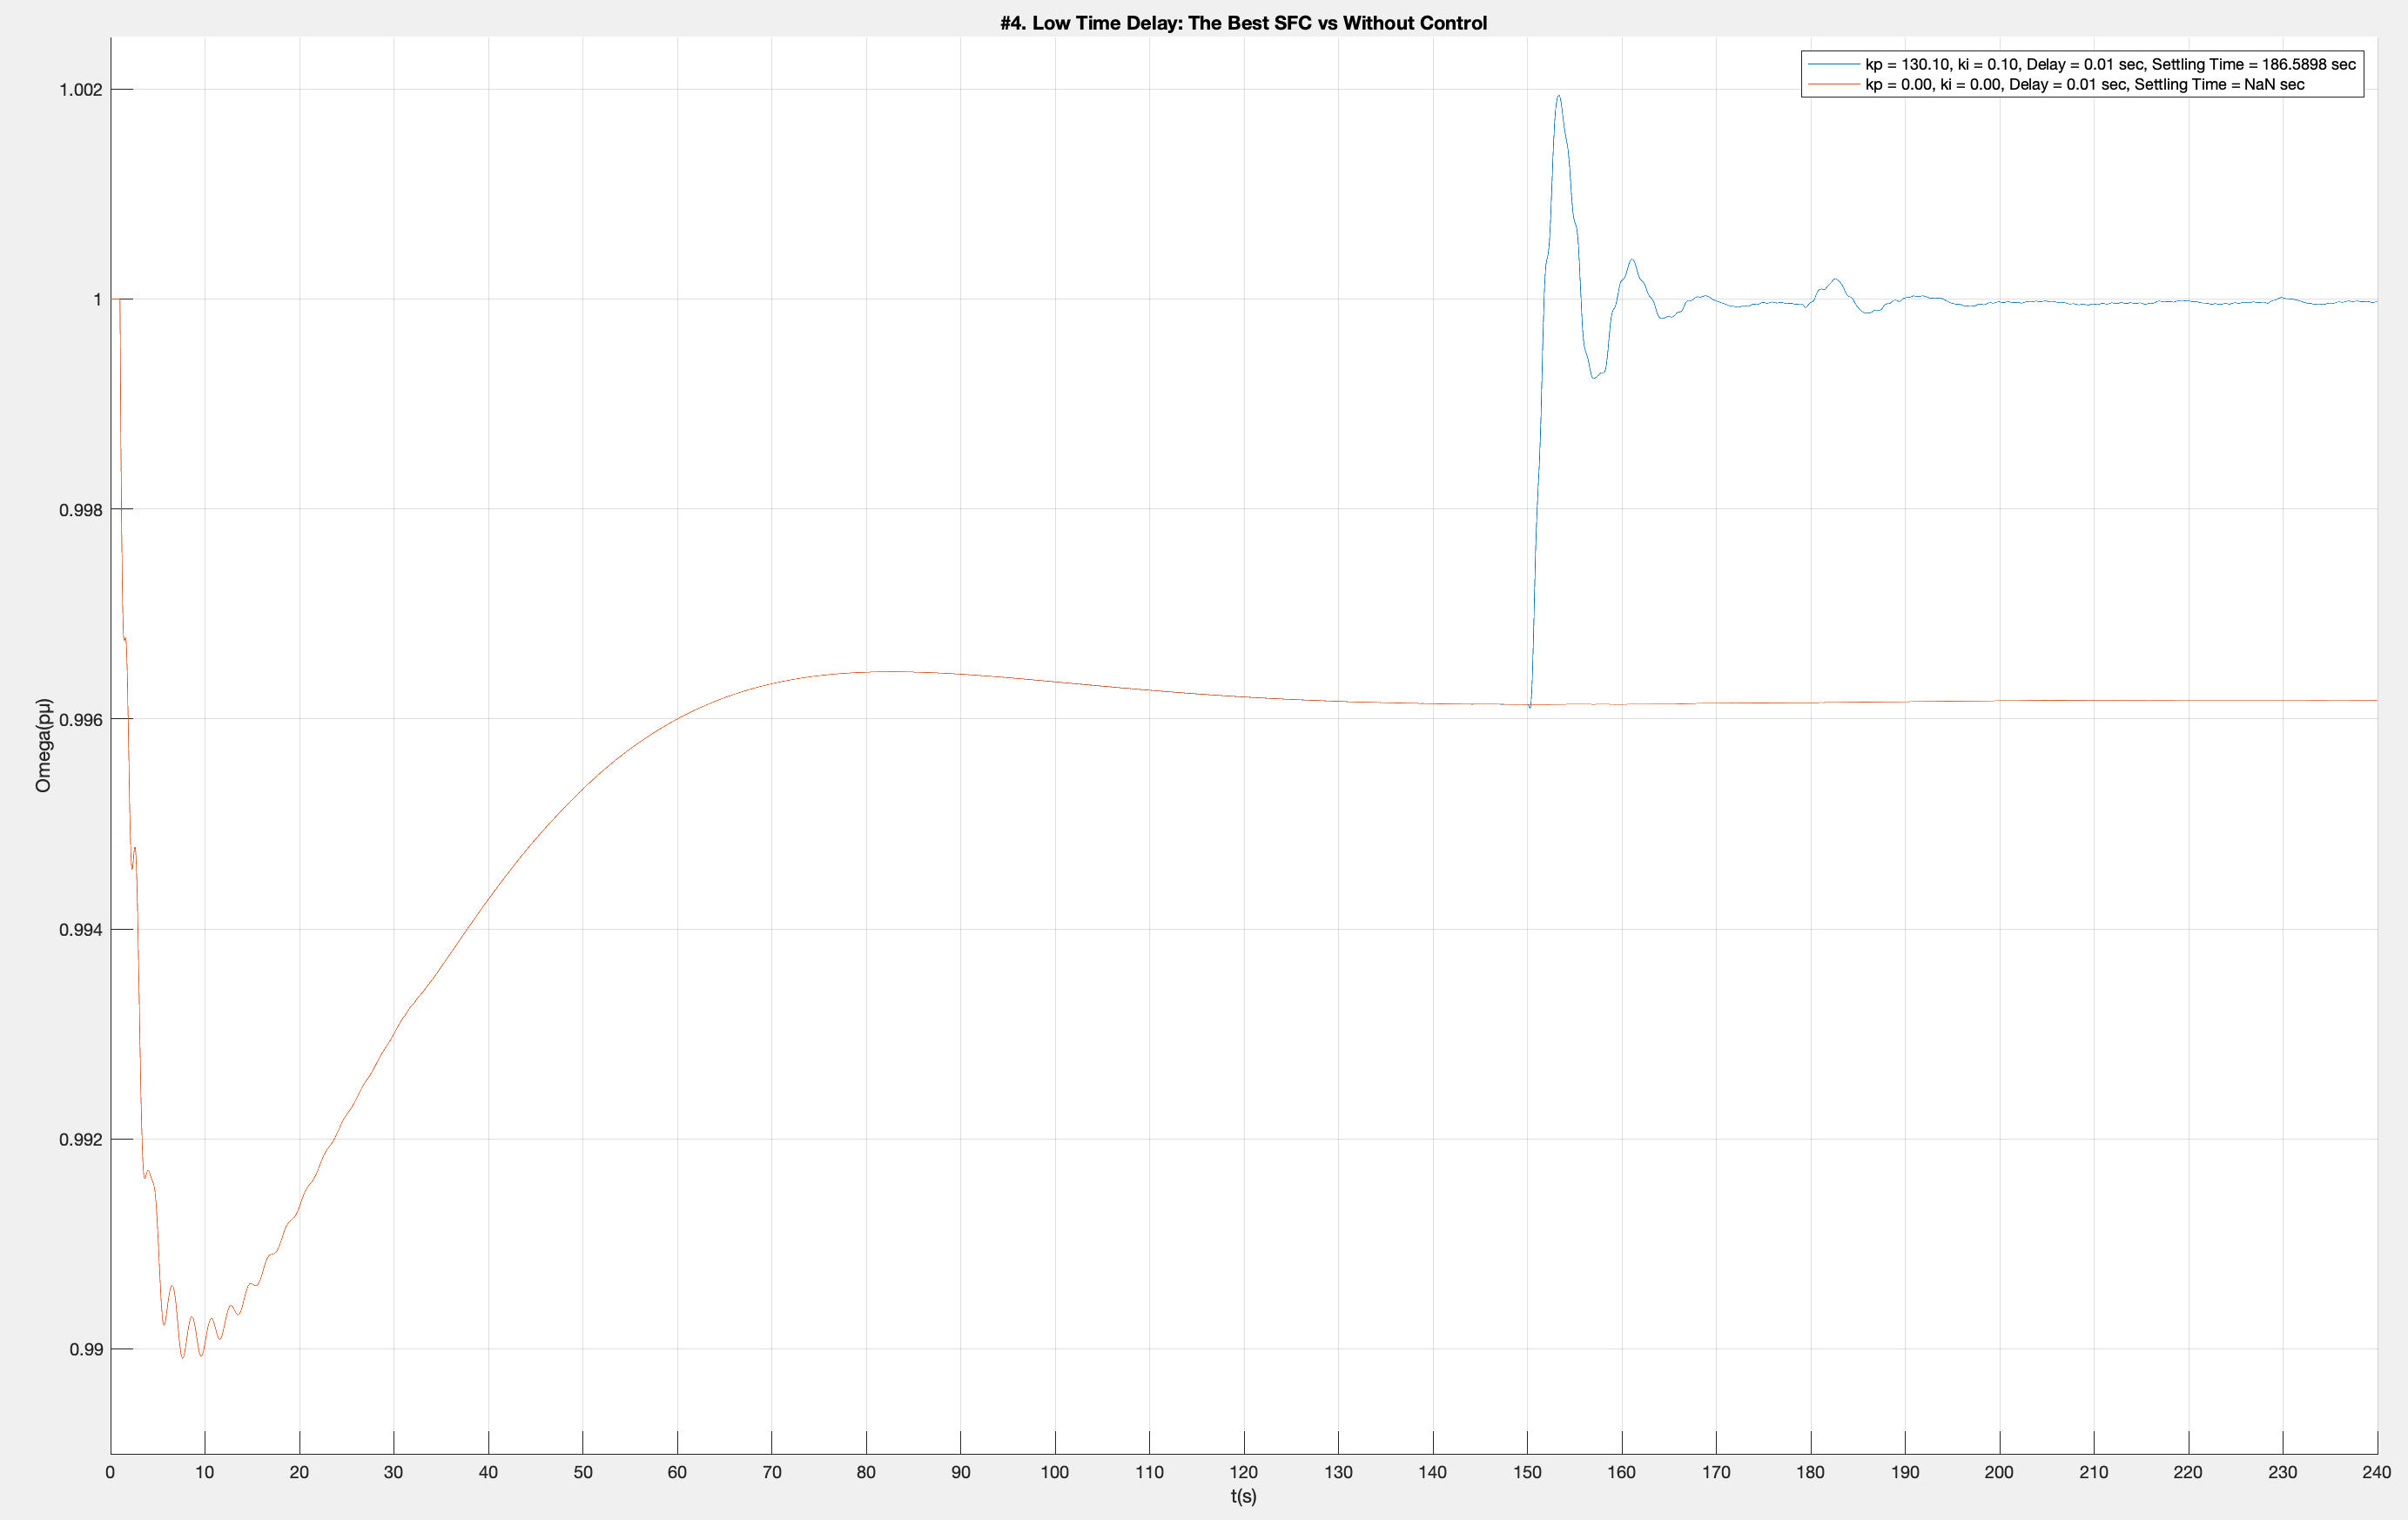
\includegraphics[width = .819\textwidth]{figure/4_4_2_best.png}
\caption{The best tuning signal}
\label{4_4_2_best}
\end{figure}